\subsection{SVM Results}
A total number of 16 different configurations of the SVM algorithm were studied, combining the values of the four kernels mentioned in the methodology section \ref{methodology-svm-sec} (linear, rbf, polynomial and sigmoid) with four different values for the $C$ value. After training and testing all these configurations of the SVM algorithm in each dataset, a previous preselection of the best models based on the accuracy were done. A Friedman test was done in order to see if there was statistical significant difference between the accuracy of the models and the one with the highest accuracy was selected for each dataset (hepatitis and mushroom). 
\newline

The best model for each dataset was trained and tested with the reduced dataset obtained after applying the methods discribed in the section \ref{reduced-methods-sec}. Consecutively, another statistical analysis was carry on in order to show which reduced method offered a better performance. A more in deep analysis of these five models can be seen in Tabla \ref{tab:svm_metrics}.

\subsubsection{Hepatitis}
Firstly, for this dataset, the five models with higher mean accuracies were selected from the 16 initial ones. The mean accuracies and the hyperparameters of those models can be consulted in Figure \ref{fig:hep-svm-1}.

\begin{figure}[t]
    \centering
    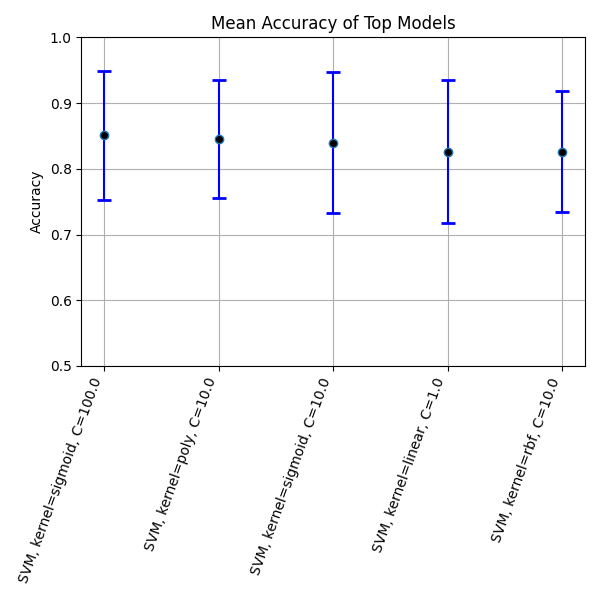
\includegraphics[width=\textwidth]{figures/svm/hepatitis/statistical_analysis_results.png}
    \caption{Mean accuracy for the five models of SVM with higher mean accuracies.}
    \label{fig:hep-svm-1}
\end{figure}


\begin{table}[h!]
\centering
\begin{tabular}{|l|c|c|c|}
\hline
\textbf{Model} & \textbf{Accuracy} & \textbf{F1 Score} & \textbf{Time (s)} \\
\hline
SVM, kernel=sigmoid, C=100.0 & 0.851 $\pm$ 0.010 & 0.91 $\pm$ 0.06 & 0.0006 $\pm$ 0.0005 \\
\hline
SVM, kernel=poly, C=10.0     & 0.84 $\pm$ 0.09 & 0.91 $\pm$ 0.05 & 0.0008 $\pm$ 0.0005 \\
\hline
SVM, kernel=sigmoid, C=10.0  & 0.84 $\pm$ 0.11 & 0.90 $\pm$ 0.07 & 0.0005 $\pm$ 0.0007 \\
\hline
SVM, kernel=linear, C=1.0    & 0.82 $\pm$ 0.11 & 0.89 $\pm$ 0.07 & 0.0011 $\pm$ 0.0006 \\
\hline
SVM, kernel=rbf, C=10.0      & 0.82 $\pm$ 0.09 & 0.89 $\pm$ 0.06 & 0.0011 $\pm$ 0.0006 \\
\hline
\end{tabular}
\caption{Performance metrics for the best five SVM models with different kernels and regularization parameters.}
\label{tab:svm_metrics}
\end{table}

The Friedman test was performed obtaining a $p-value=0.4292$ that lead us to accept the null hypothesis that there are no significant differences between the five studied models. The model with hyperparameters kernel=sigmoid and C=100.0, as it can be seen in Table \ref{tab:svm_metrics}, showed higher mean accuracy, higher mean f1 score and lower mean time in this case, thus this one will be consider for the further analysis of the reduced datasets.
\newline
The SVM model with hyperparameters kernel=sigmoid and C=100.0 was trained and tested with the reduced data samples obtained for each of the reduced methods (DROP3, EENTH and GCNN). The mean values of the studied statistical metrics for this are shown in Table \ref{tab:reduction_help}. Newly, the Friedman test was done, obtaining a $p-value= 0.0057$ for the accuracy and $p-value=0.0210$ for the f1-score. Due to these low values, the null hypothesis was neglected and a post-hoc test was implement. The chosen test was the Nemenyi test, in order to know

\begin{table}[h!]
\centering
\begin{tabular}{|l|c|c|c|}
\hline
\textbf{Reduction Method} & \textbf{Accuracy} & \textbf{F1 Score} & \textbf{Time (s)} \\
\hline
DROP3 & 0.7864 $\pm$ 0.1119 & 0.8614 $\pm$ 0.0741 & 0.0009 $\pm$ 0.0006 \\
\hline
EENTH & 0.8522 $\pm$ 0.0948 & 0.9081 $\pm$ 0.0606 & 0.0011 $\pm$ 0.0007 \\
\hline
GCNN  & 0.6443 $\pm$ 0.1271 & 0.7310 $\pm$ 0.1178 & 0.0014 $\pm$ 0.0007 \\
\hline
NONE  & 0.8507 $\pm$ 0.0987 & 0.9083 $\pm$ 0.0597 & 0.0011 $\pm$ 0.0004 \\
\hline
\end{tabular}
\caption{Performance metrics for different reduction methods for the SVM algorithm with kernel=sigmoid and C=100.}
\label{tab:reduction_hep}
\end{table}

\subsubsection{Mushroom}
